%!TEX root =  main.tex

%%%%%%%%%%%%%%%%%%%%%%%%%%%%%%%%%%%%%%%%%%%%%%%
% These are the general sections to include.  %
%                                             %
% You can alter some names, but follow the    %
% suggestions in the NSF guidelines.          %
%                                             %
% If spacing is tight, play with negative     %
% vspaces w/in the text to reduce whitespace. %
%%%%%%%%%%%%%%%%%%%%%%%%%%%%%%%%%%%%%%%%%%%%%%%

%%%%%%%%%%%%%%%%%%%%%%%%%%%%%%
% Section 1: Introduction    %
%%%%%%%%%%%%%%%%%%%%%%%%%%%%%%
\section{Introduction}
\label{intro}


% \subsection{Problem}

\mab{proposal format has too much white space between paragraphs...}

% MAB: the problem

Raw sequencing data in computational biology is increasing much faster than ever
due to high-throughput sequencing technology (HTS)~\cite{cite-sequencing-technology}, already producing
petabyte-scale datasets~\cite{cite-petabyte-scale}. Numerous applications in computational biology (\kmer
analysis~\cite{cite-kmer-analysis}, raw sequence search~\cite{cite-raw-sequence}, taxonomic classification~\cite{cite-taxonomic-classification}, and pangenomics~\cite{cite-pangenomics})
require processing raw sequencing data at petabyte scales~\cite{cite-something-or-refer-to-figure-later-in-paper}. This project aims to
build high-performance and scalable data analysis-pipelines for computational-biology applications.

As we explain (see \S{xxx} and \S{xxx}), the key technology in these pipelines is high-performance, compact, dynamic, and scalable data structures. For example:

\begin{itemize}[leftmargin=*]
%[noitemsep, leftmargin=*]

\item {\bf \Kmer analysis.}
\Kmer analysis involves representing raw sequencing data as length-$k$ subsequences called \kmers, and performing analysis on the occurrence and frequency of \kmers in the data sets; the objective is to answer questions about the genomic diversity, abundance variance, taxonomic information, etc.
\Kmer analysis is the first step in numerous computational biology pipelines, e.g., error correction, de Bruijn graph construction, raw sequence search, digital normalization, comparative genomics, genomics assembly, transcript quantification, taxonomic classification of metagenomic reads, etc~\cite{xxxx}.

Existing tools use both lossy and lossless data structures (e.g., filters vs.\ compact hash tables) to construct and store \kmer indexes~\cite{xxxx}.
For example, in raw sequencing data, singleton \kmers are erroneous and form a major fraction of the data~\cite{xxxx}. \kmer analysis tools such as  XXX use a compact filter to identify singleton \kmers and use a hash table to keep maintain the frequency count and associated metadata (e.g., prefix-suffix extension, read id, etc) about the \kmers~\cite{xxxx}.

\item {\bf Taxonomic classification.} Taxonomic classification~\cite{something} helps to identify the microbial taxon or taxa present in large-scale  metagenomic datasets coming from complex biological and environmental samples. Assigning taxonomic labels to sequencing reads is an important part of many computational genomics pipelines for metagenomics
projects.

Methods~\cite{cite-something} for taxonomic classification of metagenomic data often use hash tables to index the \kmer content of samples and quickly compare samples to prune down the search space.
Furthermore, to save space many solutions~\cite{cite-something} also employ lossy sketches (e.g., locality sensitive hashing (LSH)~\cite{cite-something}) to represent metagenomic data and perform similarity computations over sketches.
They further employ compact string indexes such as FM-index~\cite{fmindex} and compressed suffix array (CSA)~\cite{csa} to perform sequence comparison to determine exact matches among the pruned-down samples.

\item {\bf Pangenomics.}
Pangenomics involves storing the genome of a species as a sequence graph consisting of genomes of multiple individuals instead of a single linear reference. A primary goal of pangenomic variation analysis is to avoid biases that arise when treating a single genome as the reference when identifying or comparing variants across samples in a population.

Existing tools for constructing a pangenomic graph use a combination of succinct data structures (e.g., compressed bit vectors~\cite{xxx}), space-efficient, dynamic hash tables, and string data structures such as xxxxx~\cite{xxx}.

\end{itemize}

The computational-biology applications described above (and numerous others)  use a set of common data structures to perform data-analysis tasks. 
% Some of these data structures are compact but lossless and some are lossy.
Compact lossless data structures include: hash tables and succinct data structures, compact string indexes, trees.
Sketches and lossy data structures include: filters, cardinality estimators,  min-hash based sketches, other locality-sensitive hash data structures. 

% Some of these data structures are compact but lossless. For example, compact hash tables are used in \kmer analysis, taxonomic classification, and pangenomics and succinct string indexes are used in taxonomic classification and pangenomics.

% Some of these data structures are sketches or lossy representations of sets.
% For example, filters and sketches are used in taxonomic classification and large-scale raw sequence search.

% For example, \kmer analysis tools use dynamic filters and hash tables, taxonomic classification tools use dynamic hash tables and string data structures, and pangenomics tools use succinct data structures and dynamic hash tables.


The performance and scalability of the computational biology applications
depends on the space-efficiency, speed, dynamism, and scalability of the
underlying data structures they use. These data structures are also the building
blocks in many other domains, like databases, machine learning, software
systems, security applications, etc.

% and having a library of high-performance data structures will have a broader impact on applications in these domains.

%\paragraph{CPU speed and storage capacity doesn't keep up with data growth.}
\paragraph{CPU speed and RAM capacity cannot keep up with data growth.}
Unfortunately, CPU speed and RAM sizes aren't keeping up with the data growth in these and other applications. 
\prashant{Need to verify/cite these numbers.}
Although CPUs are increasing at 2--25\%/year and single-node RAM sizes are increasing at 2-11\%/year, genomics data is increasing by 100-200\%; see Figure~\ref{fig:sra_data}.
Thus, today's techniques won't work with tomorrow's data. 
Need a sentence that connects to data structures.

\setlength\intextsep{0pt}
\begin{wrapfigure}[20]{R}{4.4in}
\centering
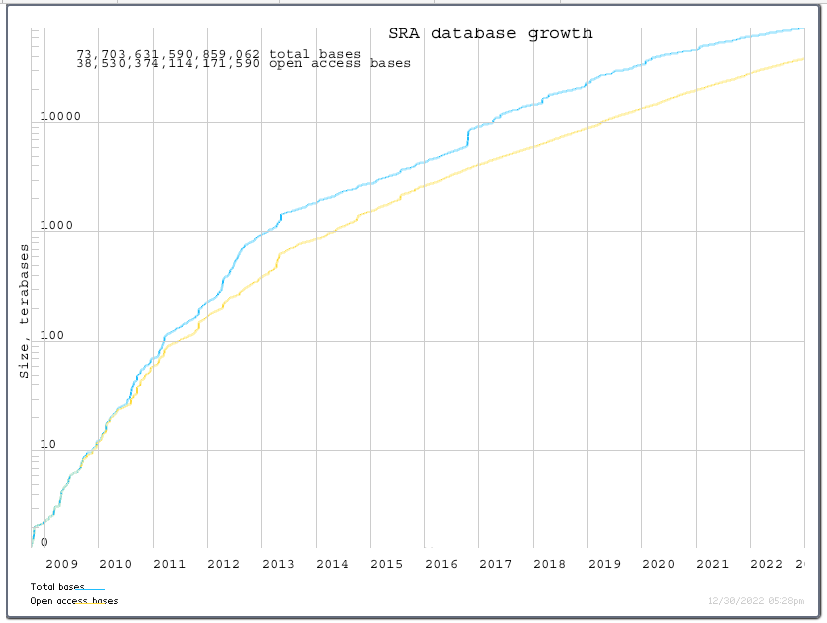
\includegraphics[width=4.4in]{images/SRA_data_growth.png}
\caption{Sequence read archive data growth over years.}
\label{fig1}
\end{wrapfigure}

% Other scaling issues: speed, data growth, what else? critical in these and other applications. 

\paragraph{GPUs and other accelerators in HPC.} 
GPUs are increasingly used in high-performance computing (HPC) because they offer a discontinuous amount of compute power and low cost compared to CPUs. 
GPUs are fast and efficient when computations are simple and straightforward and data fits in device RAM (e.g., many examples).
\prashant{add more examples.}

GPUs are used in some computational biology  applications to speed up data processing~\cite{xxx}, sequence alignment~\cite{xxx}, read-to-contig mapping~\cite{xxx}.
Give examples.

Not used in most comp bio pipelines because of GPU limitations:
%However, GPUs have a few limitations:
\begin{enumerate}[noitemsep,nolistsep]
  \item GPU device RAM is much smaller than CPU RAM; this is especially
    challenging given the data sizes in computational biology.
  \item GPUs have high contention due to thousands of threads and are
    inefficient when computations are irregular.
\end{enumerate}

These limitations affect how data structure design: 

Not used in other applications, such as ....

%Anything that involves sophisticated data structures and when memory is constrained GPUs are not currently useful.  

GPUs are not currently used for many
computational biology applications because efficient GPU data structures do not
exist.
Recent data structure advances~\cite{cite-something} show that
implementations that go beyond primitive data structures are possible on GPUs
but this work has not had much practical impact to date. A pure GPU solution is
desirable because transfer costs are high, and this is the direction being taken
in other application domains (machine learning, data science).


-- GPUs increase used in HPC, esp for easy/regular computations. Offer discontinuous growth in computational power.

-- increasingly used for data structures. E.g., in comp bio.

-- of course, most comp bio still uses CPUs.



\paragraph{This project.} 
In this project, we develop a  collection of
memory-efficient, high-performance, dynamic, and scalable GPU data structures.
We will show how to use these data structures for our target applications in comp bio, as well as some others. 
Because many of these applications require the same set of data structures, we will incorporate these data structures into a standalone library to enable easy reuse in other applications.


Solving the data growth issue via: 

-- scaling up  (via algorithms and GPUs)

-- scaling out (via distributed data structures and high-performance computing)

Four target areas

-- Theory and algorithms

-- Systems

-- High-performance computing

-- Applications









\paragraph{GPUs and other accelerators.}

In this project we envision solving these problems with a combination of  scale-up (via better algorithms and accelerators) and scale-out (distributing data and compute across multiple nodes of large high-performance computing systems).

% The rate of growth data is much higher than the growth of the CPU speeds and single-node storage capacities. CPU growth will not keep up with application demands.

Most existing applications in computational biology use CPUs to perform data  analysis. 
However, the growth of the CPU speed and capacity is slowing and at the same time data is growing faster than ever. CPU growth will not keep up with application demands.

As a consequence, a few recent tools~\cite{cite-something} have tried to scale
up using accelerators like GPUs to speed up computations. However, these tools
use only primitive data structures and as a result achieve suboptimal
performance. Some applications [cite] have also tried to scale out using
distributed memory.  However, these applications are still limited by the CPU
speed and capacity and leave performance on the table due to suboptimal
scalability of data structures.



\prashant{Assigned to Martin/Michael: Need to add theory/algorithmic challenges
to develop GPU data structures. Why is it hard to just port existing CPU data
structures to GPUs.}


\begin{enumerate}[noitemsep, leftmargin=*]
  \item Filters
  \item Hash table
  \item String data structures (suffix array, FM index, BWT)
  \item Succinct data structures (Dynamic rank-select indexes)
  \item Trees and Tries
\end{enumerate}

\subsection{Our solution}

We believe the answer to these challenges is a standalone library of
memory-efficient, high-performance, dynamic, and scalable GPU data structures
that can be directly used by computational biology applications that addresses
the needs of emerging applications, allowing them to solve the problems
described above.

The project’s novelties are: a vertical-stack approach spanning theory and
algorithms: highly-concurrent, dynamic, and distributed data structures,
systems: scale up using GPU acceleration, high-performance computing: scale out
using distributed data structures, and applications: computational biology
applications; new parallel and distributed data structures and algorithms to
exploit the massive compute on GPUs applicable to other application domains; an
API for developers to quickly and seamlessly integrate high-performance and
scalable data structures in applications.

Our team includes a highly interdisciplinary team of researchers across four
focus areas: applications (computational biology), theory and algorithms,
systems, and high-performance computing. The team is taking a holistic
theory/systems/hpc/applications co-design approach to explore four tightly
interconnected research modules.
These research modules are structured from bottom-up across the computing stack.

\begin{itemize}[noitemsep, leftmargin=*]
  \item {\bf Module 1 [theory/algorithms]:} Develop single-node GPU data structures.
    Specifically, filters, hash tables, succinct/string data structures, and
    trees. Challenges: high concurrency; being able to scale 100K threads;
    branching statements have a high cost; data movement and irregular data
    accesses are expensive. We will develop new theoretical data structures and
    algorithms that can efficiently exploit massive GPU parallelism while being
    compact and dynamic.

  \item {\bf Module 2 [Systems]:} Develop GPU data structures that can scale out of
      GPU device RAM to CPU host RAM. We will develop a memory allocator to
      seamlessly manage the GPU and CPU ram and efficiently move data across GPU
      and CPU RAMs.

    \item {\bf Module 3 [HPC]:} Develop data structures that can scale out to
      multiple-GPU nodes in a distributed computing environment. We will develop
      communication-efficient distributed versions of the above data structure
      to efficiently scale out hundreds of nodes in a HPC environment.

    \item {\bf Module 4 [Applications]:} Building high-performance and scalable
      computational biology applications by integrating GPU data structures in
      k-mer analysis, taxonomic classification, pangenomics tools.

\end{itemize}

\prashant{Section 2: State of the art, data structures (theory/systems), applications. What are the deficiencies.}\\
\prashant{Section 3: Here's what we will do. Need a concrete plan with what we are going to. Sub-problems, milestones, schedule. How the four pillars interact.}\\
\prashant{Conclusion, Broader impact, previous NSF support}


%%%%%%%%%%%%%%%%%%%%%%%%%%%%%%
% Section 2: Overview        %
%%%%%%%%%%%%%%%%%%%%%%%%%%%%%%
\section{GPU stuff}

PPoSS targets large-scale systems and we believe that GPUs will form the backbone of future large-scale, compute-intensive systems. Why?

With power constraints continuing to be the main bottleneck in increased computing performance, the superior power-performance of GPUs~\cite{Dally:2010:GCT} will make them increasingly attractive at all scales, from mobile devices to laptop and desktop computation to the largest supercomputers. The recent and extremely rapid rise of training deep neural networks for deep-learning applications~\cite{Amodei:2015:DS2,Chetlur:2014:CEP,Coates:2013:DLW,Hannun:2014:DSU}---a field led by NVIDIA GPUs and CUDA---has resulted in NVIDIA-GPU-equipped data centers in nearly every large Internet company and NVIDIA GPUs in each of the three major cloud computing providers. As well, GPUs have made enormous inroads into the largest-scale computations. GPU-centered machines dominate the top of the biannual TOP500 list~\cite{top500:nov2022}, including 7 of the top 10 (\#1 and \#3 have AMD GPUs; 157 total of the 168 GPU-centered machines have NVIDIA GPUs). In systems that have high compute requirements, GPU hardware is now ubiquitous.

The most successful GPU applications have historically been focused on highly parallel, regular workloads (e.g., training deep neural networks). What has been more challenging, and the focus of significant research effort over the past decade, has been \emph{irregular} and/or \emph{sparse} workloads that are harder to parallelize effectively. These workloads include the powerful data structures that are the focus of this proposal. While these workloads may exhibit ample parallelism and thus are potentially a good fit for the GPU, they are challenging to implement efficiently because they do not naturally map well to key GPU software design guidelines:

\begin{description}
  \item[Thread divergence] GPUs run most efficiently when neighboring threads take the same path through the code.
  \item[Memory coherence] GPU memory systems are most efficient when neighboring threads access neighboring locations in memory.
  \item[Low contention] Because GPUs have hundreds of thousands of active threads at any time, avoiding memory contention and serialization is critical to allowing GPU threads to progress and thus enabling the GPU to run at maximum efficiency.
\end{description}


-- past experience with GPU data structures





\section{Data Structures}

\setlength\intextsep{0pt}
\begin{wrapfigure}[15]{R}{4.4in}
\vspace{-5pt}
\centering
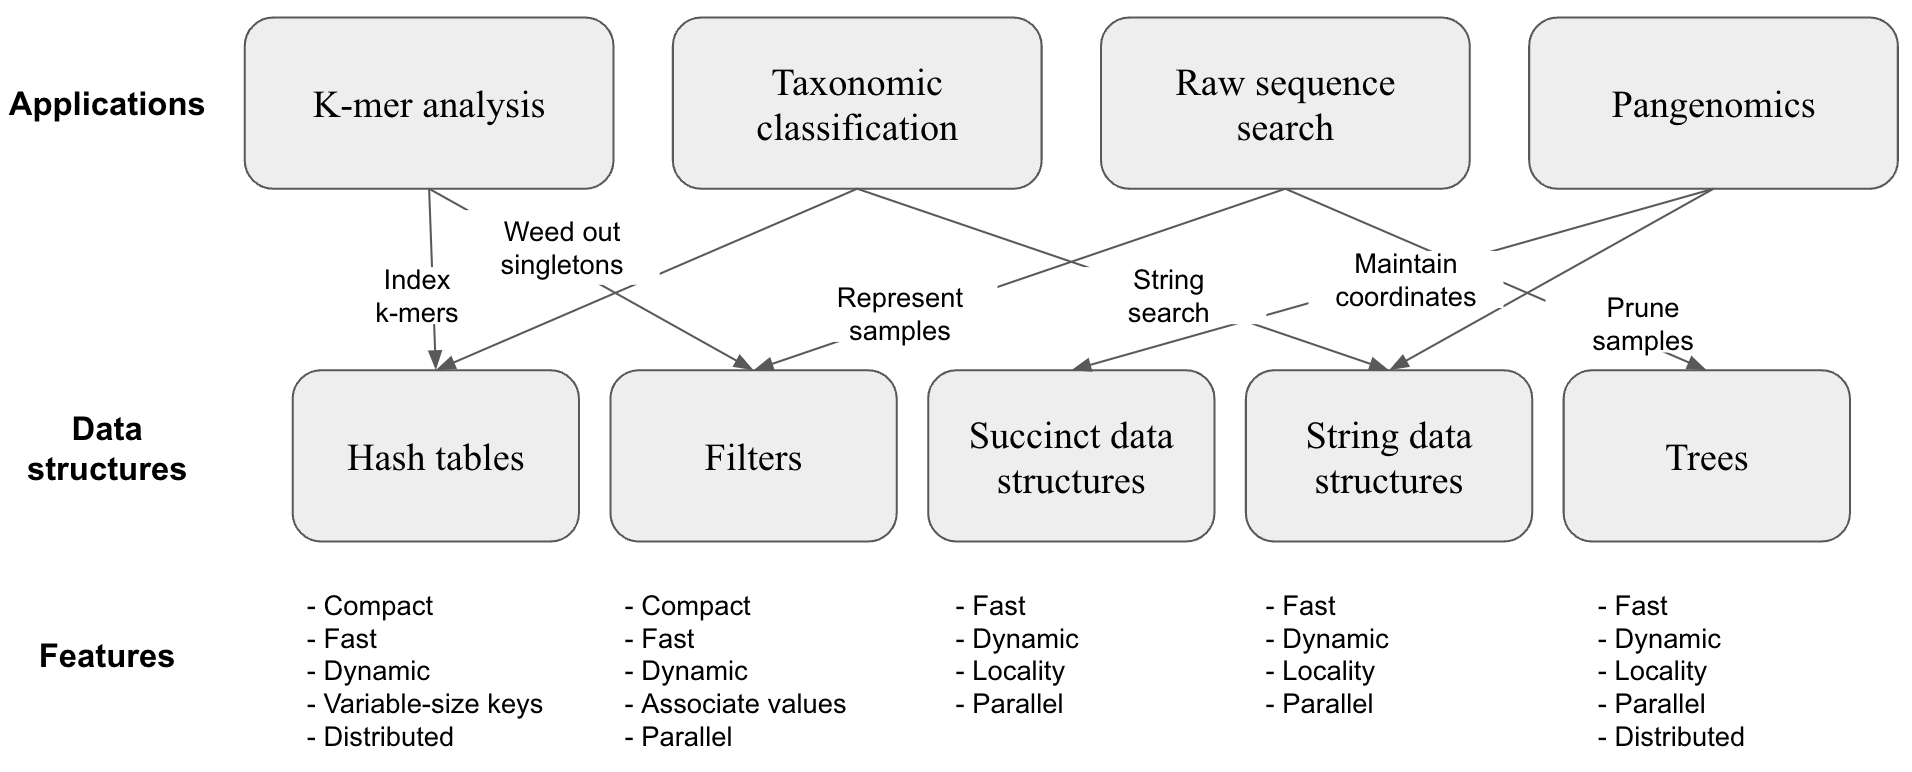
\includegraphics[width=4.4in]{images/PPoSS_App_DS.png}
\caption{Applications -- Data structures -- features.}
\label{fig1}
\end{wrapfigure}

\subsection{Filters}\label{sec:prelim}

Filter data structures can be broadly classified into \emph{static} and
\emph{dynamic}.  Static filters approximately represent a set of items that must
be known before building the filter. Examples of these filters include XOR
filters~\cite{GrafLe20} and Ribbon filters~\cite{DillingerWalzer21}. Static
filters have recently seen more advancement due their use in storage
applications, such as LSM-trees.


In this paper, we consider dynamic filters as they have wide-spread applications
in data analytics.  Dynamic filters approximately represent a set of items that
does not need to be known before the construction. Dynamic filters have seen
much more advancement in the last few decades as applications often do not know
the set of items in advance. Examples of dynamic filters are Bloom
filters~\cite{Bloom70}, quotient filters~\cite{BenderFaJo12,
PandeyBJP17b,DillingerMa09,PaghPaRa05,EinzigerFr16}, and cuckoo
filters~\cite{FanAnKa14,BreslowJ18}.

\textbf{Bloom filters} consume $\log(e)\, \opt$ space, which is roughly
$\log(e)\approx 1.44$ times more than the lower bound of $\opt + \Omega(n)$
bits~\cite{CarterFG78}. In contrast, for a set $S$ taken from a universe $U$,
where $|U|=u$, an error-free dictionary requires $\Omega(\log {u\choose n})
\approx \Omega(n \log u)$ bits. Bloom filters also incur $\errbits$ cache-line
misses on inserts and positive queries, giving them poor insertion and query
performance.

\textbf{Blocked Bloom filters}~\cite{putze2007cache} overcome the poor cache
locality of Bloom filters by constructing a series of smaller Bloom filters each
of which is small enough to fit inside a small number of cache lines. The first
hash function is used to select a block and rest of the hash functions are used
to set/test bits inside the block. However, the cache efficiency comes at the
cost of higher false-positive rate. Blocked Bloom filters have theoretically and
empirically higher (up to $5\times$) false positive rates compared to Bloom
filters. See \Cref{tab:merged_fp_space} for the empirical calculations of FP
rate.

\textbf{Quotient
filters}~\cite{Cleary84,PaghPaRa05,DillingerMa09,BenderFaJo12a,PandeyBJP17,pandeySigmod21}
represent a set approximately by compactly storing small fingerprints of the
items in the set via Robin Hood hashing~\cite{CelisLaMu85}. The quotient filter
uses $1.053 (2.125 + \log_21/\epsilon)$ bits per element, which is less than the
Bloom filter whenever $\epsilon \leq 1/64$, which is the case in almost all
applications. It supports insertion, deletion, lookups, resizing, and merging.
The counting quotient filter (CQF)~\cite{PandeyBJP17}, improves upon the
performance of the quotient filter and adds variable-sized counters to count
items using asymptotically optimal space, even in large and skewed datasets. In
the counting quotient filter, we can also associate small values with items
either by re-purposing the variable-sized counters~\cite{PandeyABFJP18Cell} to
store values or by explicitly storing small values with the remainders in the
table~\cite{PandeySMB20}.

\textbf{Cuckoo filters}~\cite{FanAnKa14,BreslowJ18} also store small
fingerprints compactly in a table. However, unlike the quotient filter that uses
Robin Hood hashing, the cuckoo filter uses cuckoo hashing to resolve collisions
among fingerprints. Cuckoo hashing uses kicking (or cuckooing) to find an empty
slot for the new item when all the slots in a bucket are occupied. This results
in a cascading sequence of kicks until the filter converges on a new stable
state. Inserts become slower as the structure becomes full, and in fact inserts
may fail if the number of kicks during a single insert exceeds a specified
threshold (500 in the author's reference implementation).

\textbf{Two-Choice filters}~\cite{pandeySigmod21} organize fingerprints
compactly in blocks similar to the cuckoo filter. However, unlike the cuckoo
filter, there is no kicking. The blocks in the two-choice filter are larger in
size ($\approx \log{n}$, where $n$ is the number of items which is usually the
size of the cache line on most machines) than the cuckoo filter and
power-of-two-choice hashing is used to reduce the variance across the blocks and
achieve a high load factor. During insertions if both blocks corresponding to a
fingerprint are full then the data structure is declared full. The
power-of-two-choice hashing enables the filter to probe exactly two cache lines
during inserts and queries and write to a single cache line during inserts.
Given the larger block sizes the vector quotient filter~\cite{pandeySigmod21}
uses quotienting (similar to the quotient filter) to organize fingerprints
inside blocks. It divides the fingerprints into a quotient and remainder part
and only stores the remainder in the slot given by the quotient. It uses two
additional metadata bits to resolve collisions among quotients.


\subsection{Analysis of filter designs}

We now look at the dynamic filters discussed in~\Cref{sec:prelim} and evaluate
them based on the GPU design principles.  Our goal is to identify the filters
that offer necessary features such as deletions, counting, and value
associations and at the same time satisfy most of the design principles.  We
will further discuss the challenges of implementing these filter on the GPUs to
achieve high speed operations.

Bloom filters are easy to implement on the GPU as they only require test and set
operations. These operations can be implemented using atomic operations and
achieve low thread divergence. However, each operation results in multiple cache
misses and therefore Bloom filters have low memory coherence. They also have
sub-optimal space usage. Moreover, Bloom filters do not support deletions,
counting\footnote{The counting Bloom filter~\cite{FanCaAl00}, a variant of the
Bloom filter, supports counting but it comes at a high space-overhead which
makes it highly inefficient in practice.}, and associating small values with
items.
% that many data analytics applications require.

Blocked Bloom filters are better suited to GPUs.  Each operation requires
probing inside a single block. They achieve low thread divergence, high memory
coherence, a high degree of parallelism, and atomic operations. Thus, blocked
Bloom filters can satisfy all the GPU design principles. However, blocked Bloom
filters have a high false-positive rate compared to Bloom filters and also do
not support necessary features like deletions and counting.

Operations in the quotient filter have high cache locality which makes it an
appropriate choice to achieve high memory coherence. However, insert operations
in the quotient filter requires shifting fingerprints which makes it harder to
use atomic operations and also results in high thread divergence. However, the
quotient filter can support all the necessary features like deletions, counting,
and associating small values with items which makes the quotient filter a highly
usable data structure that multiple applications can benefit from.

It is quite challenging to achieve high speed operations while maintaining all
of the features in a GPU implementation of the quotient filter. Geil et
al.~\cite{Geil:2018:QFA} implemented a preliminary version of the GPU quotient filter.
However, that implementation was adapted from Bender et al.'s quotient
filter~\cite{BenderFaJo12a}, which did not have all the features, like counting
and value association, and also had higher space overhead. Furthermore, Geil et
al.'s GPU-based quotient filter has implementation-specific limitations (e.g., it
supports a fixed false-positive rate and can only be sized to store less than
$2^{26}$ items) resulting in poor performance and limited scalability.

The cuckoo filter stores fingerprints in fixed size blocks. This design is
amenable to high memory coherence and low thread divergence. Atomic operations
can also be used to read and write fingerprints. However, the cascading sequence
of reads and writes to random memory locations makes the cuckoo filter hard to
implement efficiently on the GPU\@. In particular, at high load factors when the
number of kicked items becomes high, each insertion will result in very low
memory coherence. Moreover, each kicking operation results in multiple
cache-line writes. This makes it challenging to achieve high speed operations in
a GPU cuckoo filter. Moreover, cuckoo filters do not support counting and
associating small values with items.

The two-choice filter has the advantages of the cuckoo filter design. It has
fixed size blocks. Each operation requires probing into exactly two blocks, and
inserts and deletes only write into a single block. This results in low thread
divergence, high memory coherence, and a high degree of parallelism. However,
due to large block sizes a more sophisticated structure is required to maintain
fingerprints inside each block. Therefore, it is not straightforward to use
atomic operations to read or write fingerprints inside blocks. It is a
challenging task to implement a two choice filter on the GPU using atomic
operations to achieve high throughput.

\subsection{Hash tables}

Hash tables are a core data structure in many applications, including key-value
stores, databases, and big-data-analysis engines, and are included in most
standard libraries.  Hash-table performance can be a substantial bottleneck for
many applications~\cite{NealZu21,FanAn13,MetreveliZe12}.


We argue that two stricter criteria, \emph{referential stability} and \emph{low
associativity} should be optimized to yield high performance on PMEM.  As we
will see, these two goals seem to be at odds with each other, and part of the
innovation  of our hash table design is that it simultaneously achieves both.
Naturally, the third design goal for a high-performance hash table is
\emph{compactness}, but compactness also seems at odds with referential
stability and low associativity.

A hash table is said to be \defn{stable} if the position where an element is
stored is guaranteed not to change until either the element is deleted or the
table is resized~\cite{sandersstability,originalstability,KnuthVol3}.
Stability offers a number of desirable properties.  For example, stability
enables simpler concurrency-control mechanisms and thus reduces the performance
impact of locking.  Moreover, since elements are not moved, writing is
minimized, which improves PMEM performance.
expensive than reads~\cite{pmem-measurements}.

The \defn{associativity} of a hash table is the number of locations where an
element is allowed to be stored.\footnote{Associativity is often associated with
caches that restrict the locations an item may be stored in.  Here we refer to
\emph{data structural associativity}, which is a restriction on how many
locations a data structure may choose from to put an item in, even on fully
associative hardware.} The best known low-associative (DRAM) hash table is the
cuckoo hash table~\cite{Pagh:CuckooHash,PaghRo01}.  In the original design, each
element has exactly two locations in the table where it is allowed to be stored,
meaning that the associativity is two.  Low associativity yields a different set
of desirable properties---most importantly, it helps search costs. For example,
searching for an element in a cuckoo hash table is fast because there are only
two locations in the table to check.  In addition, low associativity can enable
us to further improve query performance by keeping a small amount of metadata;
see \Cref{sec:iceberght}.


In combination, stability can be used to achieve high insertion throughput in
PMEM, where writes are expensive, and low associativity can be use to achieve
high query  performance.  Furthermore, we also show how stability enables
locking and concurrency-control mechanisms to be simplified, leading to better
multithreaded scaling and simpler designs for crash consistency.

Unfortunately, there is a tension between stability and low associativity.  If a
hash table has associativity $\alpha$, and elements cannot move once they are
inserted, then an unlucky choice of $\alpha$ locations for $\alpha$ elements can
block a $(\alpha+1)$st element from being inserted.  As $\alpha$ decreases, the
probability of such an unlucky event increases.  Cuckoo hashing reduces the
probability of these bad events by giving up stability via \defn{kickout
chains}, which are chains of elements that displace each other from one location
to another. Practical implementations~\cite{LiAn14} generally increase the
number of elements that can be stored in a given location---and thus the
associativity---to reduce the kickout-chain length and increase the
maximum-allowed \defn{load factor}, i.e, the ratio of the total number of keys
in the table to the overall capacity of the table.


Similarly, there is a three-way tension between space efficiency, associativity,
and stability.  For example, cuckoo hash tables can be made stable if they are
overprovisioned so much that the kickout-chain length reaches 0.  Such
overprovisioning directly decreases space efficiency, but it also increases
associativity.  Linear probing hash tables are stable (assuming they use
tombstones to implement delete) but, as the load factor approaches 1, the
average probe length for queries goes up, increasing associativity.  Other
open-addressing hash tables have a similar space/associativity trade-off.
Chaining hash tables are stable, but they have large associativity and
significant space overheads.  CLHT~\cite{david2015asynchronized} improves query
performance despite high associativity by storing multiple items in each node,
but this further reduces space efficiency.

\subsection{B-trees}

The \btree(or B$^+$-tree\footnote{A \bplustree is a scan-optimized variant of
\btrees that stores all data records in the leaves and only pivot keys in the
internal nodes. The \bplustree is the widely implemented variant of the \btree
in real-world applications as it supports faster range
scans~\cite{mongodb,couchdb,scylladb,conway2020splinterdb,postgresql}. In this
paper, we refer to \bplustree as the \btree.})~\cite{BayerMc72} has been the
fundamental access path structure in databases and storage systems for over five
decades~\cite{Comer79,graefe2010survey}. \btrees are an extension of
self-balancing binary search trees to arbitrary fanouts (with more than two
children per node). They store elements in each node in a sorted array.  Given a
cache-line size $Z$~\cite{AggarwalVi88}, a \btree with $N$ elements and node
size $B = \Theta(Z)$ supports the point operations \proc{insert} and \proc{find}
in $O(\log_B(N))$ cache-line transfers in the I/O model~\cite{AggarwalVi88}.
\btrees are one of the top choices for in-memory indexing~\cite{ZhangChOo15} due
to their cache efficiency though they were initially introduced for indexing
data stored on disk~\cite{BayerMc72}. In this paper, we study and improve the
performance of in-memory \btrees.

\btrees are especially popular in databases and file systems because they
support logarithmic point operations (inserts and finds) and efficient range
operations (range queries and scans) that read blocks of
data~\cite{Knuth98,rodeh2013btrfs}.  They are also extensively used as the
in-memory index in many popular databases such as MongoDB~\cite{mongodb},
CouchDB~\cite{couchdb}, ScyllaDB~\cite{scylladb}, PostgreSQL~\cite{postgresql},
and SplinterDB~\cite{conway2020splinterdb}.

\subsection{Succinct data structures}

\section{Theory Notes}

\mab{this is still just for private consumption. I'm writing down notes for the issues and I'm also going to be writing some research problems.}


\section{Applications}

\subsection{MetaHipMer}

Metagenome assembly involves reconstructing long contiguous sequences ({\it
contigs}) of genetic material from short input {\it reads}. These reads are
strings of bases (the DNA alphabet A,C,G,T) of length 150 to 250 that are
produced by gene sequencing machines.  For metagenomes, these reads are
extracted from environmental samples (e.g. gut bacteria, or a soil sample) that
contain the genes of potentially thousands of microbes, existing at varying
abundances.  The reads are error prone (typically about 0.24\% error per base)
and sequencing is done multiple times to ensure every region of genetic material
is covered with some error free sequences.

In the approach used by MetaHipMer, the reads are first divided into overlapping
substrings of fixed length {\it k}, called {\it $k$-mers}, which are then used
to form a de Bruijn graph~\cite{CompeauPeTe11}. In a de Bruijn graph, the
vertices are $k$-mers and edges connect any two $k$-mers that have an overlap of
$k-1$ bases. These vertices are stored in a hash table that is distributed
across all the compute processes.  The size of the hash table is dependent on
the number of unique $k$-mers.  Traversal of the de Bruijn graph enables the
construction of the contigs (longer sequences).  This approach is more efficient
than an all-to-all alignment of the reads, which would be prohibitive for the
size of typical metagenome datasets (up to billions of reads).

Forward and backward extensions of the $k$-mer and the counts of those
extensions are also maintained in the hash table along with the $k$-mer.
Information regarding the extensions and their counts is critical to identifying
correct paths in the de Bruijn graph and requires 28 to 52 bytes (depending on
$k$) to store each $k$-mer.

To ensure accurate contigs, the $k$-mers that occur only once (singletons) are
treated as errors and dropped. In a typical set of metagenome reads, 70 to 80\%
of unique $k$-mers are singletons, but they still need to be stored and counted
in the distributed hash table. In the default MetaHipMer implementation, storing
the unique $k$-mers is the most memory intensive part of the computation and can
be roughly an order of magnitude larger than the input data.  The space required
to store the $k$-mers can be much larger than the size of the original raw
dataset (up to $10\times$ larger) as $k$-mers contain a lot of redundant
information due to their overlaps.

The distributed hash table in MetaHipMer is implemented as a collection of local
hash tables, one per process, with communication happening via UPC++ remote
procedure calls (RPCs). In the hash table insertion phase, the $k$-mers are
aggregated, dispatched over the network, and inserted in bulk into the local
hash tables, which are running on GPUs. Using GPUs boosts performance, but
further constrains memory (e.g. the Summit supercomputer~\cite{VazhkudaiDBG18}
has an aggregate of 96GB GPU memory and 512GB CPU memory per node).

MetaHipMer runs on distributed systems with multiple nodes, and each node could
have multiple GPUs, e.g. Summit has 6 GPUs per node. To utilize all the GPUs on
a node, MetaHipMer maps the UPC++ processes to the GPUs in a round robin
fashion, so multiple processes will share each GPU using the Nvidia
Multi-Process Service (MPS). On a Summit node there will be 42 processes (one
per core) and hence there will be 7 processes per GPU\@. Using the MPS has the
benefits of simplicity, because there is no inter-GPU communication required,
and it improves performance by increasing the utilization of the GPUs.

\Cref{fig:mhm-kmer} shows different parts of the $k$-mer analysis phase in
MetaHipMer. In the standard pipeline, all $k$-mers are counted in the hash table
and then a separate phase is required to purge all the singleton $k$-mers.

\subsection{\Kmer distribution}

\begin{wraptable}[15]{r}[0.01in]{4.5in}
\centering
%\resizebox{\columnwidth}{!}{%
    \begin{tabular}{c | c | c | c | c | c}
    \toprule
    {\bf Dataset} & \multicolumn{5}{c}{\bf Percentage singleton $k$-mers} \\
    \midrule
    & $K=21$ & $k=33$ & $k=55$ & $k=77$ & $k=99$ \\
    \midrule
    WA &  66 & 73 & 76 & 78 & 78  \\
    Rhizo &  67 & 75 & 80 & 83 & 85  \\
    Tymeflies & 63 & 62 & 67 & 69 & 71 \\
    \bottomrule
    \end{tabular}
 %   }
    \caption{Distribution of singleton $k$-mers in metagenomic datasets with different values of $k$.}
    \label{tab:kmer-dist}
\end{wraptable}

\Cref{tab:kmer-dist} shows the distribution of singleton \kmers in three
different metagenomic datasets. Singleton \kmers form a majority fraction of
the total number of distinct \kmers. The distribution often depends on the
sequencing depth and the size of $k$. The larger value $k$ results in larger
fraction of singleton \kmers. This is due to the higher probability of seeing
an erroneous base in the \kmer given the higher value of $k$. The erroneous
bases result in singleton \kmers.

Weeding out singleton \kmers before inserting them in the hash table to count
is critical in any \kmer analysis phase to reduce the memory usage of the
counting phase. These singleton $k$-mers can also be pruned from the hash table
after the counting phase. However, that results in the high peak memory usage
and much slower running time.

Using a space-efficient filter to weed out singleton \kmers helps to reduce
the memory pressure on the counting hash table thereby reducing the peak memory
usage and increased run time. See~\cref{fig:mhm-kmer}.


%%%%%%%%%%%%%%%%%%%%%%%%%%%%%%
% Section 3: Research Plan   %
%%%%%%%%%%%%%%%%%%%%%%%%%%%%%%
\section{Research Methodology}


\subsection{Filters}
Applications require this:
\begin{itemize}
    \item Filters needs to associate small values with each item
    \item filter need to scale to large datasize and being able to saturate the GPU parallelism
    \item Support deletion of items to save space
    \item Being able to dynamically resize the filter
\end{itemize}

\subsection{Hash tables}
\begin{itemize}
    \item More locality and in turn performance
    \item variable-length keys and values support
    \item Being able to dynamically resize the filter
\end{itemize}

\subsection{Succinct/string string data structures}
SDSL library is heavily used across comp biology. 

\begin{itemize}
    \item We need to build succinct data structures that are GPU-architecture aware.
    \item Making succinct data structures dynamic is hard. There is a trade off between space-efficiency and dynamism.
    \item We need to prove some lower-bounds to support dynamic operations while being succinct.
    \item We need to understand the empirical overheads to achieve dynamic operations. 
\end{itemize}

\subsection{Trees}
\begin{itemize}
    \item Tree are relatively easier to distribute
    \item Tree have a fair amount if locality
    \item 
\end{itemize}

\subsection{Distributed data structures}

\begin{itemize}
    \item more locality
    \item communication efficiency --- trade off between latency and bandwidth
    \item communication pattern -- all-to-all 
    \item global coherence 
\end{itemize}

\subsection{Spanning the entire hardware/software/network stack.}

\john{I don't think we want to say ``hardware'' here anywhere because we don't address it anywhere. ``Software stack'' makes more sense to me.}

\paragraph{Coverage areas.} Data structures are ubiquitous throughout the
hardware/software stack, as a way to connect heterogeneous components within a
system and to scale-out in data-center-scale applications.  AT has become a
bottleneck, but redesigning AT is tantamount to renegotiating the division of
labor among system components---requiring a closely knit team and an approach
that weighs the costs and benefits holistically.
Our team has the needed expertise:

% \begin{itemize}[noitemsep,nolistsep]
\begin{description}
  \item[Theory and Algorithms (PIs Bender and Farach-Colton)]
    Bender and Farach-Colton have written numerous
    top-tier theory
    publications~\cite{DBLP:conf/stoc/BenderFK19,DBLP:conf/focs/BenderFGJM018,DBLP:conf/soda/BenderCCFJT19,DBLP:conf/soda/AfshaniBFFGT17,DBLP:conf/pods/BenderFJMMPX17,DBLP:conf/stoc/BenderKPY16,DBLP:conf/soda/BenderFGKM17,DBLP:conf/pods/BenderBJKMPSSZ16}
    and have, along with collaborator Conway, made significant contributions in
    the theory of hashing and its
    applications~\cite{BenderFaGo18,BenderFaJo12,BenderFaJo11,PandeyBeJo17,PandeyAlBe18,PandeyBeJo18,PandeyBeJo17c,DBLP:conf/icalp/ConwayFS18}.


    \item[GPU Systems (PIs Owens and Pandey)] Owens's research program in GPU computing~\cite{Owens:2007:ASO,Owens:2008:GC} spans nearly 20 years and includes representative research advances in fundamental algorithms~\cite{Sengupta:2007:SPF}, data structures~\cite{Lefohn:2006:GGE,Alcantara:2009:RPH}, performance engineering~\cite{Zhang:2011:AQP}, programming models~\cite{Gupta:2012:ASO, Tzeng:2010:TMF}, and applications~\cite{Wang:2017:GGG}.

    \item[High-Performance Computing (PIs Bender, Farach-Colton, Owens, and
        Pandey)] Bender, Farach-Colton, Owens, and Pandey have
      written a number of top-tier papers in HPC~\cite{pandey2020timely,bender2017two,eckstein2015pebbl,agrawal1989four,bender2008communication,greenberg1999enabling},
      and had considerable impact on HPC practice.  PI Bender's and Phillips
      work in HPC has focused on scheduling and  won a joint R\&D 100 Award for
      processor scheduling and allocation algorithms, which were licensed by
      Cray and incorporated into SLURM.  PIs Bender and Farach-Colton's company
      Tokutek deployed software to manage metadata in a large cloud storage
      service. Owens led the first implementation of MPI on GPUs~\cite{Stuart:2009:MPO:withouturl,Stuart:2011:EMT}, the first multi-GPU MapReduce~\cite{Stuart:2011:MMO}, and more recent work on scalable graph analytics on HPC machines~\cite{Pan:2018:SBS,Pan:2017:MGA,Chen:2022:SIP}.

    \item[Large-scale genomics (PIs Bender, Farach-Colton, and Pandey)]

\end{description}


\paragraph{Target distributed applications and systems, and the heterogeneous platforms on which they run.}

Accelerating data analyses will benefit all big-data application domains.  In
this proposal, we will primarily focus on \textbf{genomics} applications. We will
start with scalable graph processing applications (e.g.,
Graph500~\cite{graph500}), and will then explore data-serving applications
(e.g., key-value stores~\cite{lakshman2010cassandra, papyruskv-kim-sc17} and
databases~\cite{MySQL}), followed by data-analytics frameworks (e.g., Apache
Spark~\cite{Zaharia:Spark:HotCloud10}). To understand the benefits and the
implications on massively parallel scale-out systems, we will study traditional
scientific simulations, such as molecular simulations (e.g., GTC~\cite{GTC}) and
biomolecular workflows (e.g., Gromacs~\cite{GROMACS}), followed by modern HPC ML
suites (e.g., MLPerf~\cite{MLPerf}).

\paragraph{Notions of Scale.}  Our proposed work address several notions of
scale.  First, virtual memory is a major bottleneck for scaling individual
machines to larger memories and CPU counts.  Without a principled redesign of
VM, additional RAM and cores will be of diminishing value.  Second, our work
supports \emph{scale-out} cloud applications, which rely on naming, placing, and
translating accesses to resources that are distributed across multiple machines.
%Currently, if one needs to do complex operations on sensitive data in the
%cloud, there is no secure and sensible option other than scaling out across
%multiple SGX enclaves.
If successful, our work will improve the performance of each node, as well as
the working-set size each node can handle, potentially improving both by orders
of magnitude.  Third, this includes scaling from only CPUs, to {\em
heterogeneous} computing accelerators, such as GPUs and FPGAs, at rack-scale or
greater.  Prior work has demonstrated that data movement and address translation
in GPUs is a first-order performance issue~\cite{pichai:gpu,
power:gpummu,rossbach:ptask}. Further, cloud computing infrastructure, such as
Microsoft's Catapult, aggregate these accelerators and move data  at the
granularity of racks, not single nodes~\cite{putnam:catapult}.  These
accelerators are evolving rapidly and in ways that are hard to anticipate; thus,
a principled design is necessary to efficiently scale to new classes of future,
unknown compute hardware.


\subsection{A component of your plan}


\setlength\intextsep{0pt}
\begin{wrapfigure}[20]{R}{2.4in}
\vspace{-5pt}
\centering
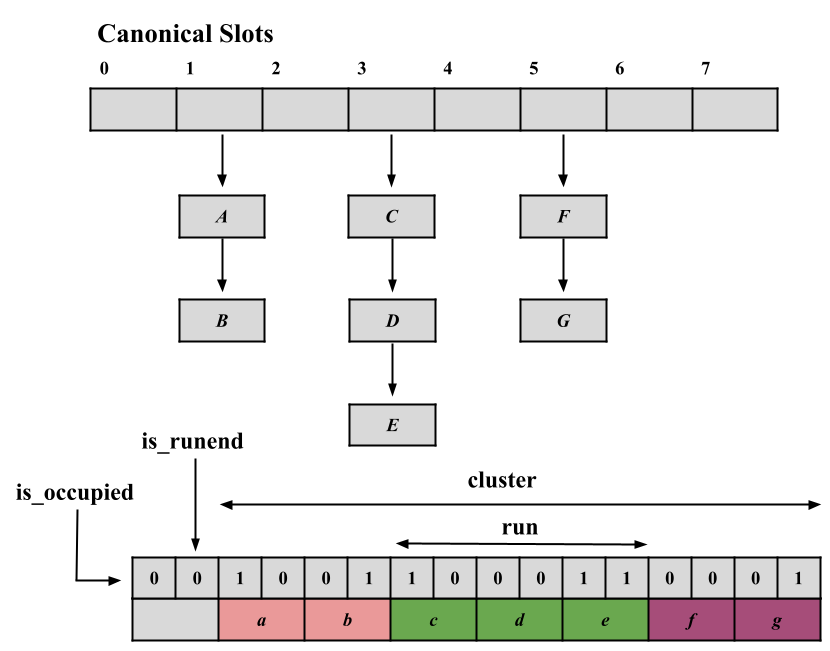
\includegraphics[width=2.4in]{images/canonical_slots}
\caption{Quotient filter block diagram.}
\label{fig1}
\end{wrapfigure}




\begin{wraptable}[15]{r}[0.01in]{4.5in}
\label{table1}
\caption{A sample table wrapped by text.}
\begin{center}
\vspace{-10pt}
\scriptsize
\begin{tabular}{  c  c  c  }
\hline
\hline
Stability & $M_u$ & $M_{\tau}$ \\
\hline\hline\\
Neutral & $\cfrac{z}{z_\Delta} - \cfrac{\ln(z/z_o)}{\ln(z_\Delta/z_o)}$ & $\cfrac{z}{z_\Delta} - \cfrac{1}{\ln(z_\Delta/z_o)}$\\\\
\hline \\
Stable & $\left(1 - \cfrac{\Psi}{2}\right)\cfrac{z}{z_\Delta} - \left(1 - \cfrac{\Psi_\Delta}{2}\right)
\left(\cfrac{\ln(z/z_o)-\Psi}{\ln(z_\Delta/z_o)- \Psi_\Delta}\right)$ & $\cfrac{z}{z_\Delta} - \cfrac{\left(1 - \cfrac{\Psi_\Delta}{2}\right)}{\ln(z_\Delta/z_o) - \Psi_\Delta}$\\\\
\hline \\
Unstable & $\cfrac{4}{3}\left[\left(\cfrac{1-x^3}{1-x_{\Delta}^{4}}\right) -  \left(\cfrac{1-x_{\Delta}^3}{1 - x_{\Delta}^{4}}\right)\left(\cfrac{\ln(z/z_o)-\Psi}{\ln(z_\Delta/z_o)- \Psi_\Delta}\right)\right]$ & $\cfrac{z}{z_\Delta} - \cfrac{\cfrac{4}{3}\left(\cfrac{1-x_{\Delta}^3}{1 - x_{\Delta}^{4}}\right)}{\ln(z_\Delta/z_o) - \Psi_\Delta}$\\\\
\hline
\hline
\end{tabular}
\end{center}
\end{wraptable}



% I found it useful to include a summary of the proposed work
% given in each subsection to help out reviewers.
\subsubsection{Specific tasks for this research component}
\begin{itemize}
\setlength\itemsep{0em}
\item Do a thing and blow your mind
\item Question your life choices
\item Drink coffee
\end{itemize}

\begin{center}
\begin{minipage}{.3\textwidth}
\begin{equation}
 \bar u = \bar u_{ll} + u_* \beta M_{u} \label{new_u}
\end{equation}
\end{minipage}
\begin{minipage}{.36\linewidth}
\begin{equation}
  \tau_{xz} = u_* u_{*ll} + \kappa u_*^2 \beta M_{\tau} \label{new_tau} \mbox{ ,}
\end{equation}
\end{minipage}
~\\Sample equations that consume minimal space.
\end{center}



%%%%%%%%%%%%%%%%%%%%%%%%%%%%%%
% Section 4: Management Plan %
%%%%%%%%%%%%%%%%%%%%%%%%%%%%%%
\section{Time Line and Management Plan}

\begin{table}[H]
\label{table1}
\renewcommand{\arraystretch}{0}
\caption{Project schedule.  PIs are Person One (P1), Person Two (P2), graduate student is GS, and the undergraduate student is US\@. Time frame gives the year each activity will occur.}
\scriptsize
\begin{tabularx}{\textwidth}{Y c c }
\hline
\hline
\textbf{Research Activity} & \textbf{Personnel} & \textbf{Time Frame}\\
\hline
Perform a task that sounds impressive & P2, US & Y1 \T\\
Perform another super-amazing task & P1, US & Y1 \T\\
Perform something else that may not be as sexy as the other things & P2, GS & Y1 \T\\
Wonder why you are such a terrible programmer & P1, US & Y1 \T\\
Analyze the results and stuff & P1, P2, SS & Y1,Y2 \T\\
Take the day off and grill some meat & P1, P2, SS & Y1,Y2 \T\\
Present findings at scientific meetings and publish results in peer-reviewed journals & P1, P2, US, GS & Y1, Y2, Y3\T\B\\
\hline
\hline
\end{tabularx}
\end{table}

%%%%%%%%%%%%%%%%%%%%%%%%%%%%%%
% Section 5: Science Merit   %
%%%%%%%%%%%%%%%%%%%%%%%%%%%%%%
\section{Scientific Merit}


%%%%%%%%%%%%%%%%%%%%%%%%%%%%%%
% Section 6: Impact/Outreach %
%%%%%%%%%%%%%%%%%%%%%%%%%%%%%%

\section{Broader Impacts}
\label{broadimpacts}
\vspace*{-8pt}

This project will have direct impacts on research and education through access to simulation data products, student training, and K-12 outreach.

\vspace{4pt}
\noindent \underline{\textit{Data Access}}: Maybe write about you will make data available.

\vspace{4pt}
\noindent \underline{\textit{Student Training}}: Write about how you will train students.

\vspace{4pt}
\noindent \underline{\textit{Some Other Outreach}}: Write about more outreach.

\vspace{4pt}
\noindent \underline{\textit{Dissemination}}: Write about how you will disseminate results (i.e., journal articles, workshops, etc).

%%%%%%%%%%%%%%%%%%%%%%%%%%%%%%
% Section 7: Prior NSF Work  %
%%%%%%%%%%%%%%%%%%%%%%%%%%%%%%
\section{Results from Prior NSF Support}

\noindent \emph{\underline{Person One}}: No NSF support in the past five years \newline

\noindent The most relevant prior NSF award to the proposed project for
\underline{Person Two} (Co-PI) is: (a) NSF PDM \#\#\#\#\#\#\#, \$000,000,
MM/DD/YY to MM/DD/YY; (b) Title: Super Cool Project That Got Funded; (c)
Accomplishments related to the \textbf{intellectual merit} of this research project
include something something. The \textbf{broader impacts} include outreach at many
levels. Something Something. To date, the grant has funded one post-doc and 1000
graduate students. The project has also involved 500 undergraduate students. (d)
To date this project has resulted in 100 conference presentations, one million
journal publications (cite them) with one under review (cite it) and two in
preparation with well-developed drafts.

For PI Owens, the NSF award whose outcomes most influenced this grant was the recently completed NSF Algorithms in the Field award CCF-1637442, ``AitF: Collaborative Research: Theory and Implementation of Dynamic Data Structures for the GPU'', with Mart\'{i}n Farach-Colton (Rutgers). This work focused on the design and implementation of GPU-friendly, dynamic, general-purpose data structures.

\paragraph{Intellectual Merit.} In this AitF award, the PIs designed and built numerous dynamic data structures that marked their first implementation on GPUs: linked lists and hash tables~\cite{Ashkiani:2018:ADH}, log-structured merge trees~\cite{Ashkiani:2018:GLA}, B-trees~\cite{Awad:2019:EAH}, quotient filters~\cite{Geil:2018:QFA}, and dynamic graphs~\cite{Awad:2020:DGO}. RXMesh's mesh data structure~\cite{Mahmoud:2021:RAG} was a result of this award. As well, the PIs recently designed and implemented the fastest GPU static hash tables~\cite{Awad:2023:AAI}.

\paragraph{Broader Impacts.} Each of the abovementioned projects is available as open-source software, a significant reason why this work is highly cited. The dynamic graphs were integrated into Gunrock~\cite{Awad:2020:DGO,Wang:2017:GGG}, which subsequently was selected as the performance reference for the DARPA HIVE program and in turn integrated into NVIDIA's open-source RAPIDS framework for data science. Finally, NVIDIA's cuCollections library currently only supports static and dynamic maps but these were both influenced by the PIs' work and we expect as this library grows, it will incorporate the abovementioned work either directly or as the basis for NVIDIA's implementation and improvements.


% \nocite*
% don't do that
